\documentclass[aspectratio=169,11pt]{beamer}
\usepackage[T1]{fontenc}
\usepackage{lmodern,amsmath,amssymb,mathtools,bm,booktabs,array,graphicx,tikz}
\usetikzlibrary{arrows.meta,positioning,calc,decorations.pathreplacing,patterns}
\definecolor{ink}{HTML}{17344D}\definecolor{accent}{HTML}{087E8B}\definecolor{pale}{HTML}{EDF5F5}\definecolor{gold}{HTML}{AD6B19}
\providecommand{\dd}{\,\mathrm{d}}\providecommand{\R}{\mathbb{R}}
\providecommand{\E}{\mathbb{E}}\providecommand{\Var}{\operatorname{Var}}
\providecommand{\Cov}{\operatorname{Cov}}\providecommand{\diag}{\operatorname{diag}}
\providecommand{\norm}[1]{\left\lVert#1\right\rVert}
\providecommand{\abs}[1]{\left|#1\right|}
\usefonttheme{professionalfonts}
\setbeamercolor{normal text}{fg=black,bg=white}
\setbeamercolor{frametitle}{fg=ink,bg=white}
\setbeamercolor{title}{fg=ink}\setbeamercolor{structure}{fg=accent}
\setbeamercolor{block title}{fg=ink,bg=pale}\setbeamercolor{block body}{fg=black,bg=pale!40}
\setbeamercolor{alerted text}{fg=accent}
\setbeamerfont{frametitle}{size=\Large,series=\bfseries}
\setbeamerfont{title}{size=\LARGE,series=\bfseries}
\setbeamertemplate{navigation symbols}{}
\setbeamersize{text margin left=.7cm,text margin right=.7cm}
\setbeamertemplate{frametitle}{\vspace{.18cm}\insertframetitle\par\vspace{.1cm}{\color{accent}\hrule height .6pt}\vspace{.12cm}}
\newcommand{\notestarget}{notes.pdf}\newcommand{\noteslabel}{Notes}
\setbeamertemplate{footline}{\hspace{.7cm}\color{ink}\scriptsize Mathematical Modeling\quad\href{\notestarget}{\noteslabel}\hfill\insertframenumber\,/\,\inserttotalframenumber\hspace{.7cm}\vspace{.18cm}}
\setbeamercovered{invisible}
\hypersetup{pdfauthor={Zan Ahmad},pdftitle={Pulsatile circulation: changing compliance and self-consistent valves},pdfpagemode=UseNone}
\begin{document}
\begin{frame}[plain]\vfill
{\small\color{accent} Mathematical Modeling \quad Lecture 4}\par\medskip
{\raggedright\hyphenpenalty=10000\exhyphenpenalty=10000\LARGE\bfseries\color{ink} Pulsatile circulation: changing compliance and self-consistent valves}\par\bigskip
Zan Ahmad\par\smallskip
{\small Fall 2024}\par\vfill\end{frame}
\renewcommand{\notestarget}{notes.pdf\#note-six-compartments-and-a-closed-volume-account}
\begin{frame}[t,fragile,label=slide-conservation-storage-and-link-laws]{Conservation, storage, and link laws}
\[\dot{\mathbf V}=B\mathbf Q,\qquad V_i=V_{d,i}+C_i(t)P_i.\]\pause{}\[Q_{\rm resistor}=G\Delta P,\qquad Q_{\rm valve}=G[\Delta P]_+.\]\par\medskip Dots use time $\tau$ in minutes; displayed seconds satisfy $t=60\tau$.
\end{frame}
\renewcommand{\notestarget}{notes.pdf\#note-six-compartments-and-a-closed-volume-account}
\begin{frame}[t,fragile,label=slide-topology-of-the-closed-circulation]{Topology of the closed circulation}
PV $\to$ LV $\to$ SA $\to$ SV $\to$ RV $\to$ PA $\to$ PV.\pause{}\par Four valves are directed; two tissue resistances are bidirectional. Every transfer has two endpoint signs.
\end{frame}
\renewcommand{\notestarget}{notes.pdf\#note-six-compartments-and-a-closed-volume-account}
\begin{frame}[t,fragile,label=slide-hydraulic-time-units]{Hydraulic time units}
\[[C]=\mathrm L/\mathrm{mmHg},\quad[Q]=\mathrm L/\mathrm{min}.\]\pause{}\[10\frac{\mathrm L}{\mathrm{min}}\frac{.06\ \mathrm s}{60\ \mathrm s/\mathrm{min}}=.010\ \mathrm L.\]
\end{frame}
\renewcommand{\notestarget}{notes.pdf\#note-pumping-by-a-time-dependent-storage-relation}
\begin{frame}[t,fragile,label=slide-shared-ventricular-phase]{Shared ventricular phase}
\[\phi(t)=ft/60,\qquad T=60/f=.75\ \mathrm s\quad(f=80).\]\pause{} One phase drives both ventricular compliance functions. The baseline has no rate feedback.
\end{frame}
\renewcommand{\notestarget}{notes.pdf\#note-pumping-by-a-time-dependent-storage-relation}
\begin{frame}[t,fragile,label=slide-product-differentiation-in-the-storage-law]{Product differentiation in the storage law}
\[V=V_d+CP\quad\Rightarrow\quad\dot V=C\dot P+\dot CP.\]\pause{} At fixed volume, $CP$ is constant.
\end{frame}
\renewcommand{\notestarget}{notes.pdf\#note-pumping-by-a-time-dependent-storage-relation}
\begin{frame}[t,fragile,label=slide-isovolumic-pressure-change]{Isovolumic pressure change}
\[V-V_d=.10\ \mathrm L,\quad C=.002\ \mathrm L/\mathrm{mmHg}\Rightarrow P=50\ \mathrm{mmHg}.\]\pause{} Halve $C$: the pressure doubles at unchanged volume.
\end{frame}
\renewcommand{\notestarget}{notes.pdf\#note-valve-flow-and-the-pressure-inequalities}
\begin{frame}[t,fragile,label=slide-ideal-valve-inequalities]{Ideal-valve inequalities}
\[Q=G[P_{\rm up}-P_{\rm down}]_+.\]\pause{} Open: $\Delta P\geq0$. Closed: $\Delta P\leq0$ and $Q=0$. Equality gives zero flow.
\end{frame}
\renewcommand{\notestarget}{notes.pdf\#note-an-implicit-equation-for-pressure}
\begin{frame}[t,fragile,label=slide-backward-difference-of-stored-volume]{Backward difference of stored volume}
\[\frac{C^{n+1}\mathbf P^{n+1}-C^n\mathbf P^n}{h}=-L_S\mathbf P^{n+1}.\]\pause{} Each pressure multiplies its matching compliance.
\end{frame}
\renewcommand{\notestarget}{notes.pdf\#note-an-implicit-equation-for-pressure}
\begin{frame}[t,fragile,label=slide-fixed-state-matrix-problem]{Fixed-state matrix problem}
\[\boxed{(C^{n+1}+hL_S)\mathbf P^{n+1}=C^n\mathbf P^n.}\]\pause{} A candidate open valve contributes to both diagonal and off-diagonal entries of $L_S$.
\end{frame}
\renewcommand{\notestarget}{notes.pdf\#note-an-implicit-equation-for-pressure}
\begin{frame}[t,fragile,label=slide-positive-definiteness]{Positive definiteness}
\[\mathbf z^T(C+hL_S)\mathbf z=\sum_iC_i z_i^2+h\sum_{\{i,j\}}G_{ij}(z_i-z_j)^2>0.\]\pause{} Positive compliance removes the pure Laplacian nullspace.
\end{frame}
\renewcommand{\notestarget}{notes.pdf\#note-a-complete-valve-state-iteration}
\begin{frame}[t,fragile,label=slide-nested-time-and-valve-iterations]{Nested time and valve iterations}
Guess states $\to$ solve $\to$ test inequalities.\pause{}\par Hold the old pressures, old/new compliances, and clock fixed throughout this inner iteration.
\end{frame}
\renewcommand{\notestarget}{notes.pdf\#note-a-complete-valve-state-iteration}
\begin{frame}[t,fragile,label=slide-an-inconsistent-closed-candidate]{An inconsistent closed candidate}
$C^{\rm old}=(1,1)$, $P^{\rm old}=(2,1)$, $C^{\rm new}=(.5,1)$.\pause{}\par Closing the valve $1\to2$ gives $(4,1)$, violating $P_1\leq P_2$.
\end{frame}
\renewcommand{\notestarget}{notes.pdf\#note-a-complete-valve-state-iteration}
\begin{frame}[t,fragile,label=slide-a-consistent-open-candidate]{A consistent open candidate}
For $hG=1$,\[\begin{bmatrix}1.5&-1\\-1&2\end{bmatrix}\begin{bmatrix}P_1\\P_2\end{bmatrix}=\begin{bmatrix}2\\1\end{bmatrix}.\]\pause{}\[P_1=2.5>P_2=1.75,\qquad .5P_1+P_2=3.\]
\end{frame}
\renewcommand{\notestarget}{notes.pdf\#note-valve-flow-and-the-pressure-inequalities}
\begin{frame}[label=slide-aortic-flow-and-pressure-crossing-panel-1]{Ventricular and arterial pressures}
\centering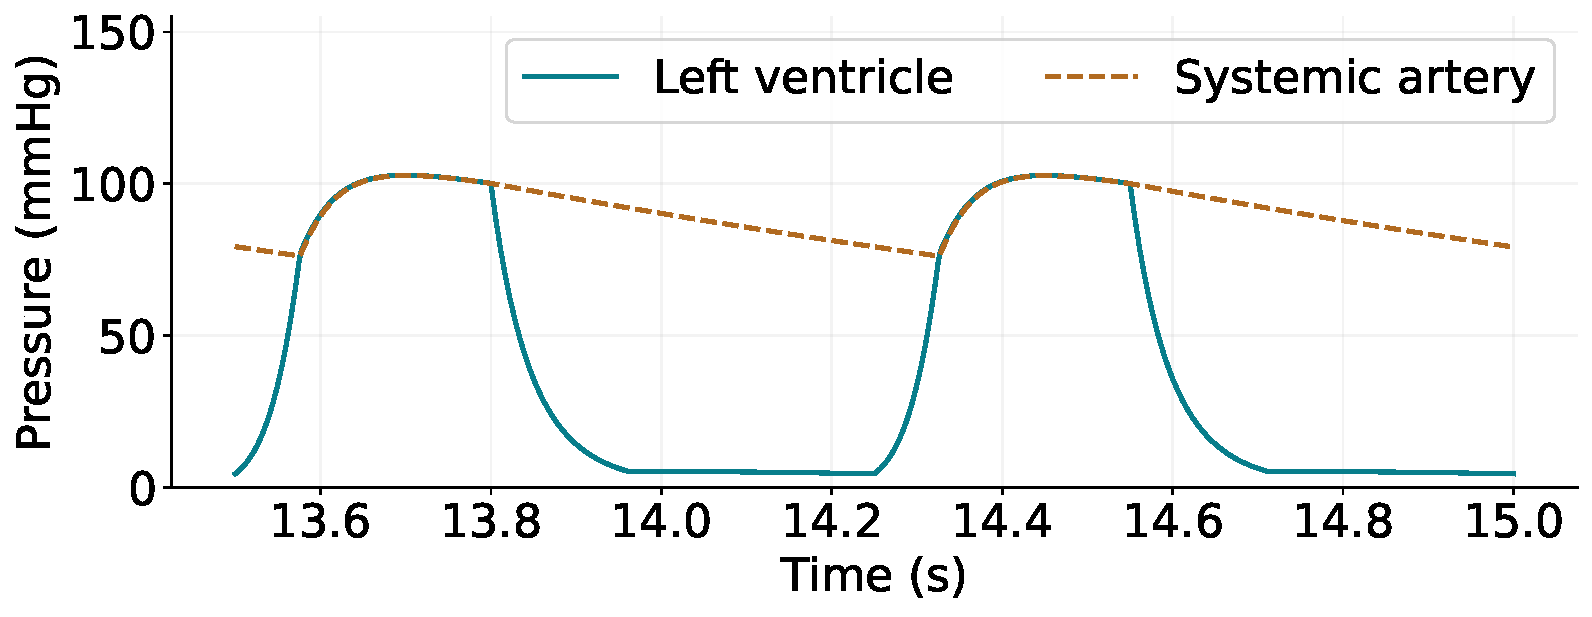
\includegraphics[width=.98\linewidth,height=.69\textheight,keepaspectratio]{presentation-figures/ventricular-arterial-pressure-panel.pdf}\end{frame}
\renewcommand{\notestarget}{notes.pdf\#note-valve-flow-and-the-pressure-inequalities}
\begin{frame}[label=slide-aortic-flow-and-pressure-crossing-panel-2]{Aortic valve flow at the same times}
\centering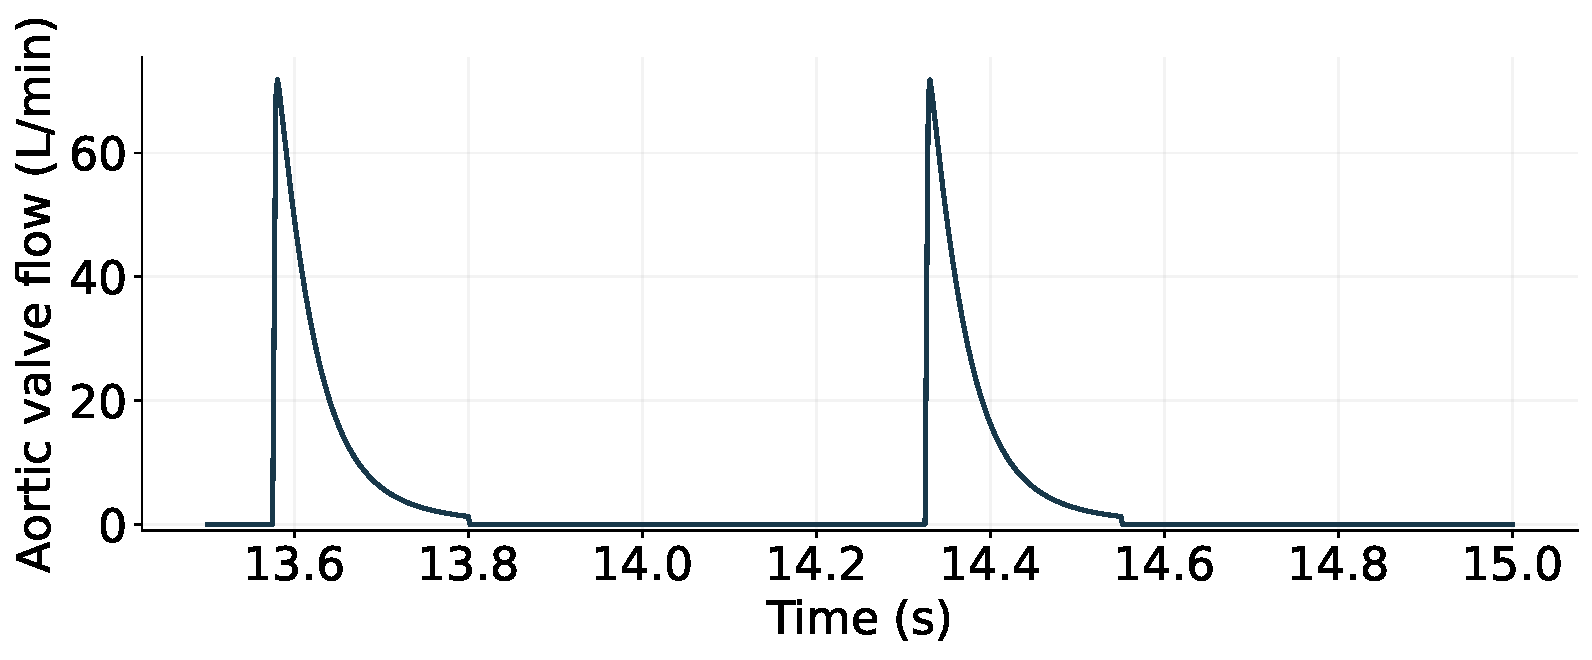
\includegraphics[width=.98\linewidth,height=.69\textheight,keepaspectratio]{presentation-figures/aortic-flow-panel.pdf}\end{frame}
\renewcommand{\notestarget}{notes.pdf\#note-valve-flow-and-the-pressure-inequalities}
\begin{frame}[t,fragile,label=slide-aortic-flow-and-pressure-crossing]{Aortic flow and pressure crossing}
$Q_{\rm Ao}>0$ requires $P_{\rm LV}>P_{\rm SA}$.\pause{}\par The figure is a finite startup calculation, not a claim of exact periodicity.
\end{frame}
\renewcommand{\notestarget}{notes.pdf\#note-matched-state-residuals-and-conservation}
\begin{frame}[label=slide-discrete-total-volume-conservation-figure]{Discrete total-volume conservation}
\centering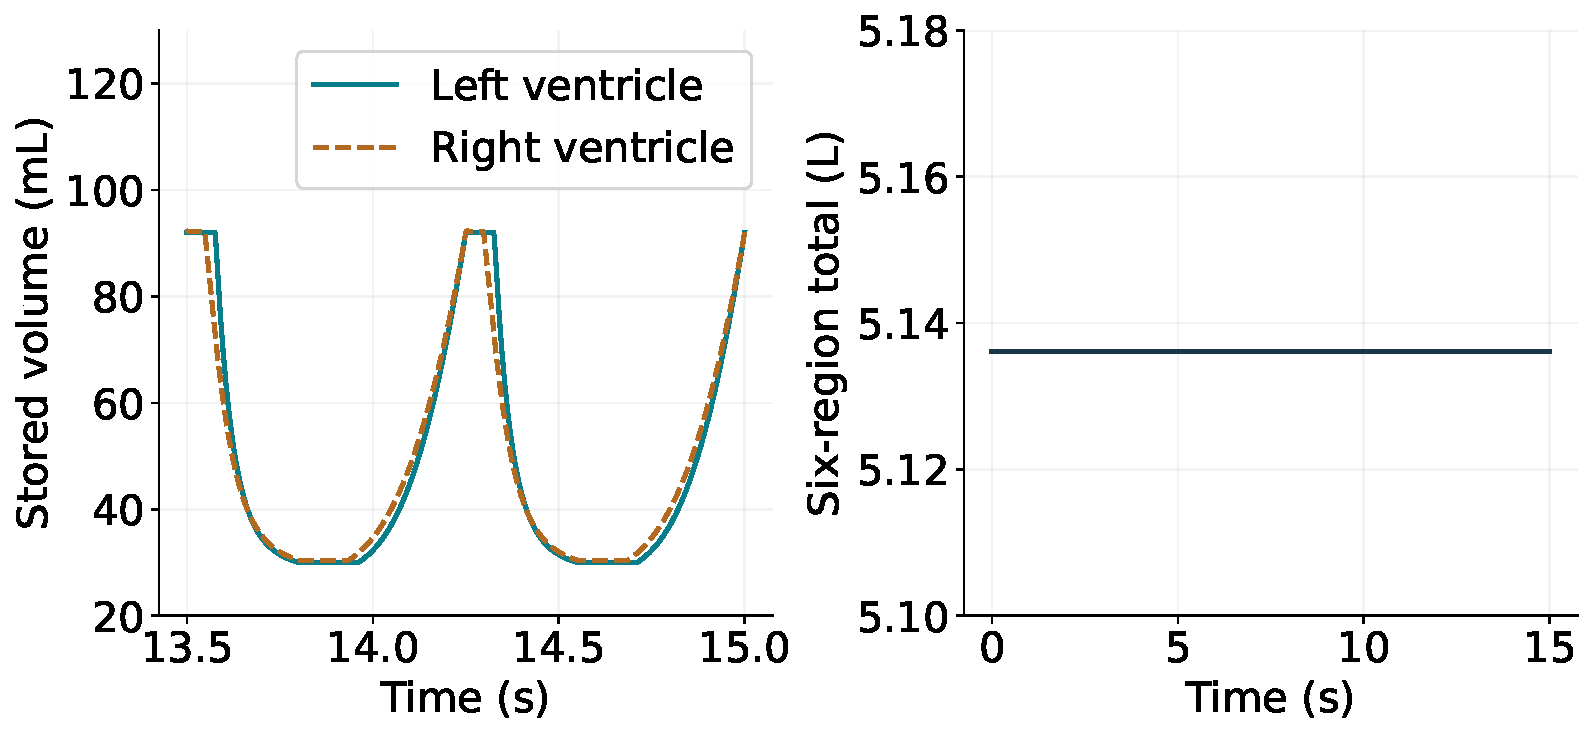
\includegraphics[width=.98\linewidth,height=.69\textheight,keepaspectratio]{changing-storage.pdf}\end{frame}
\renewcommand{\notestarget}{notes.pdf\#note-matched-state-residuals-and-conservation}
\begin{frame}[t,fragile,label=slide-discrete-total-volume-conservation]{Discrete total-volume conservation}
\[\mathbf1^TL_S=0\Rightarrow\sum_iC_i^{n+1}P_i^{n+1}=\sum_iC_i^nP_i^n.\]\pause{} Fixed unstressed volumes complete the volume total.
\end{frame}
\renewcommand{\notestarget}{notes.pdf\#note-matched-state-residuals-and-conservation}
\begin{frame}[t,fragile,label=slide-local-residual-and-storage-reconstruction]{Local residual and storage reconstruction}
\[\mathbf r^{n+1}=\frac{\mathbf V^{n+1}-\mathbf V^n}{h}-B\mathbf Q^{n+1}.\]\pause{} Also verify valve inequalities and $V_i=V_{d,i}+C_i(\phi)P_i$.
\end{frame}
\renewcommand{\notestarget}{notes.pdf\#note-matched-state-residuals-and-conservation}
\begin{frame}[t,fragile,label=slide-parameter-provenance-and-numerical-refinement]{Parameter provenance and numerical refinement}
Baseline $R_s=17.86$; reference source $R_s=8$.\pause{}\par Halving the step tests time sensitivity. Changing resistance changes the physical model. Update $G_s=1/R_s$ consistently.
\end{frame}
\end{document}
